\documentclass[10pt]{article}
\usepackage[utf8]{inputenc}
\usepackage{geometry}
\usepackage[sort]{natbib}
\usepackage{pxfonts}
\usepackage{graphicx}
\usepackage{setspace}
\usepackage{hyperref}
\usepackage{lineno}
\usepackage{authblk}

\doublespacing
\linenumbers

\title{\textit{Supplementary materials for} Fitness tracking reveals task-specific associations between
  memory, mental health, and exercise}
\author[1, $\star$]{Jeremy R. Manning}
\author[1,2]{Gina M. Notaro}
\author[1]{Esme Chen}
\author[1]{Paxton C. Fitzpatrick}
\affil[1]{Dartmouth College, Hanover, NH}
\affil[2]{Lockheed Martin, Bethesda, MD}
\affil[$\star$]{Address correspondence to jeremy.r.manning@dartmouth.edu}

\begin{document}
\maketitle


\begin{figure}[p]
\centering
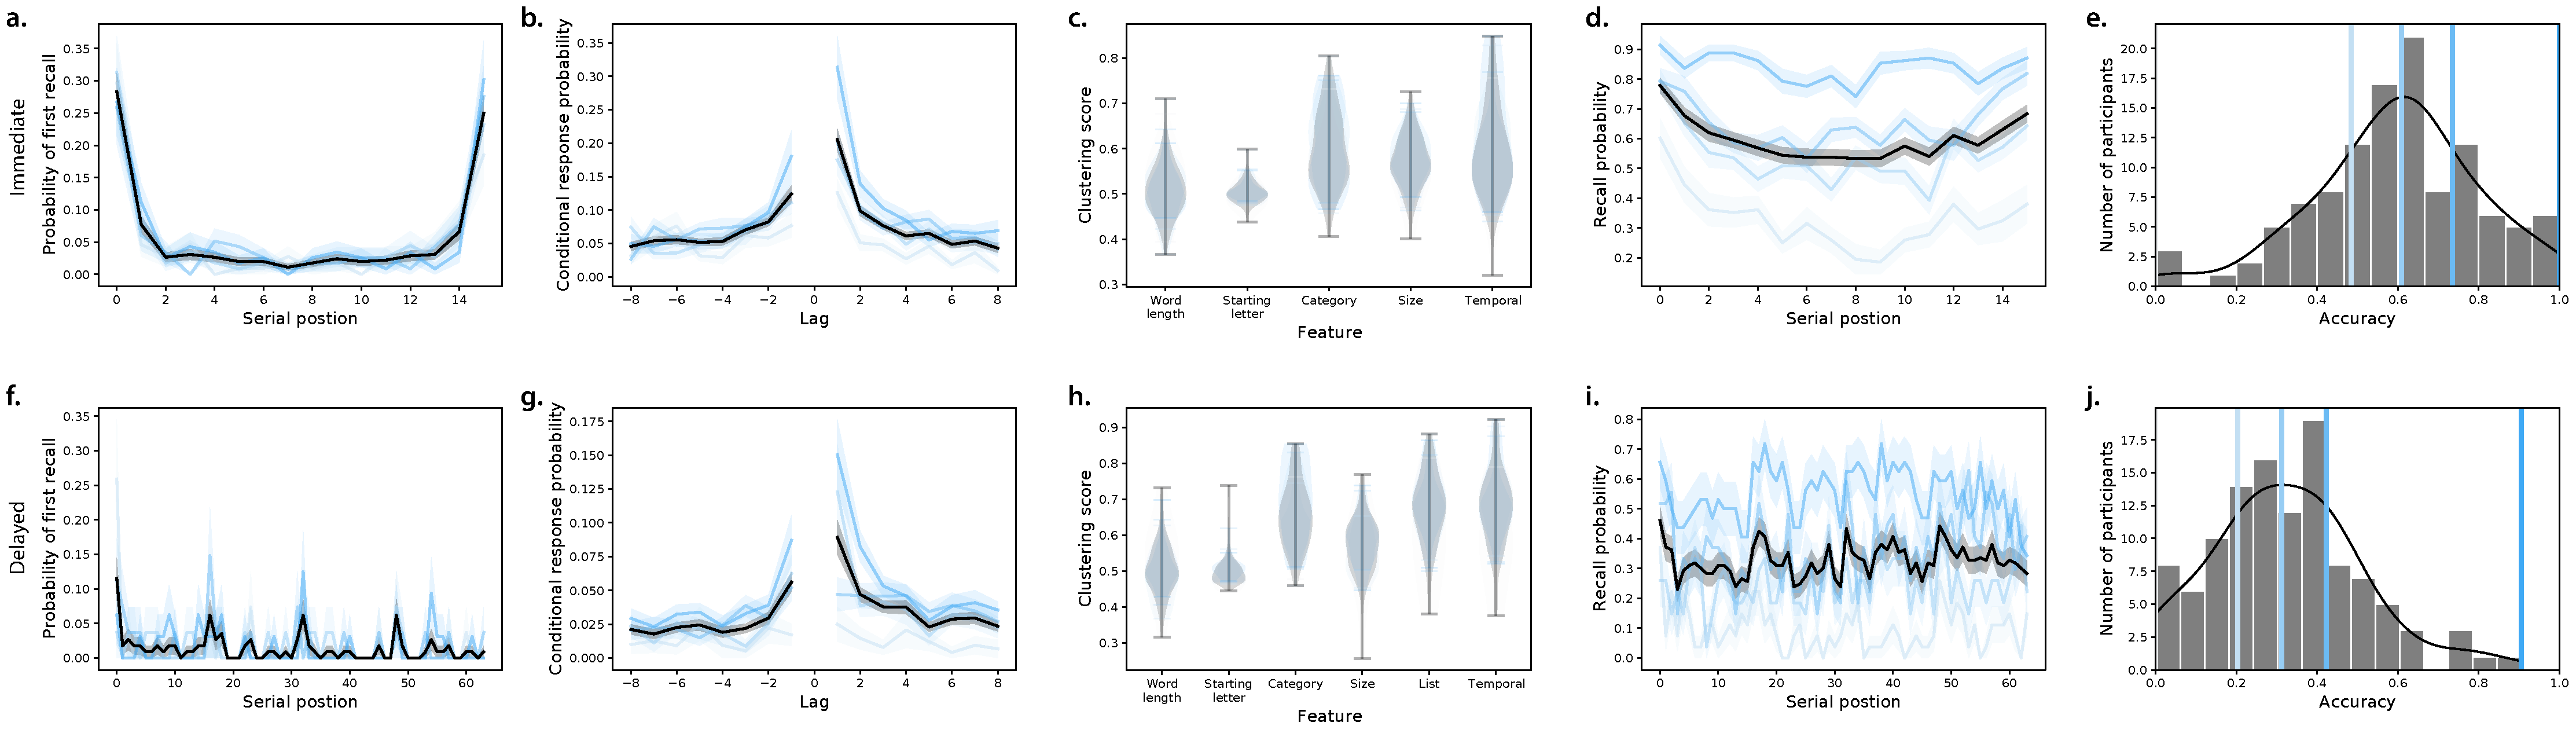
\includegraphics[width=1\textwidth]{figs/free_recall_behavior}
\caption{\textbf{Free recall behavioral results.}}
\label{fig:fr_behavioral}
\end{figure}

\begin{figure}[p]
\centering
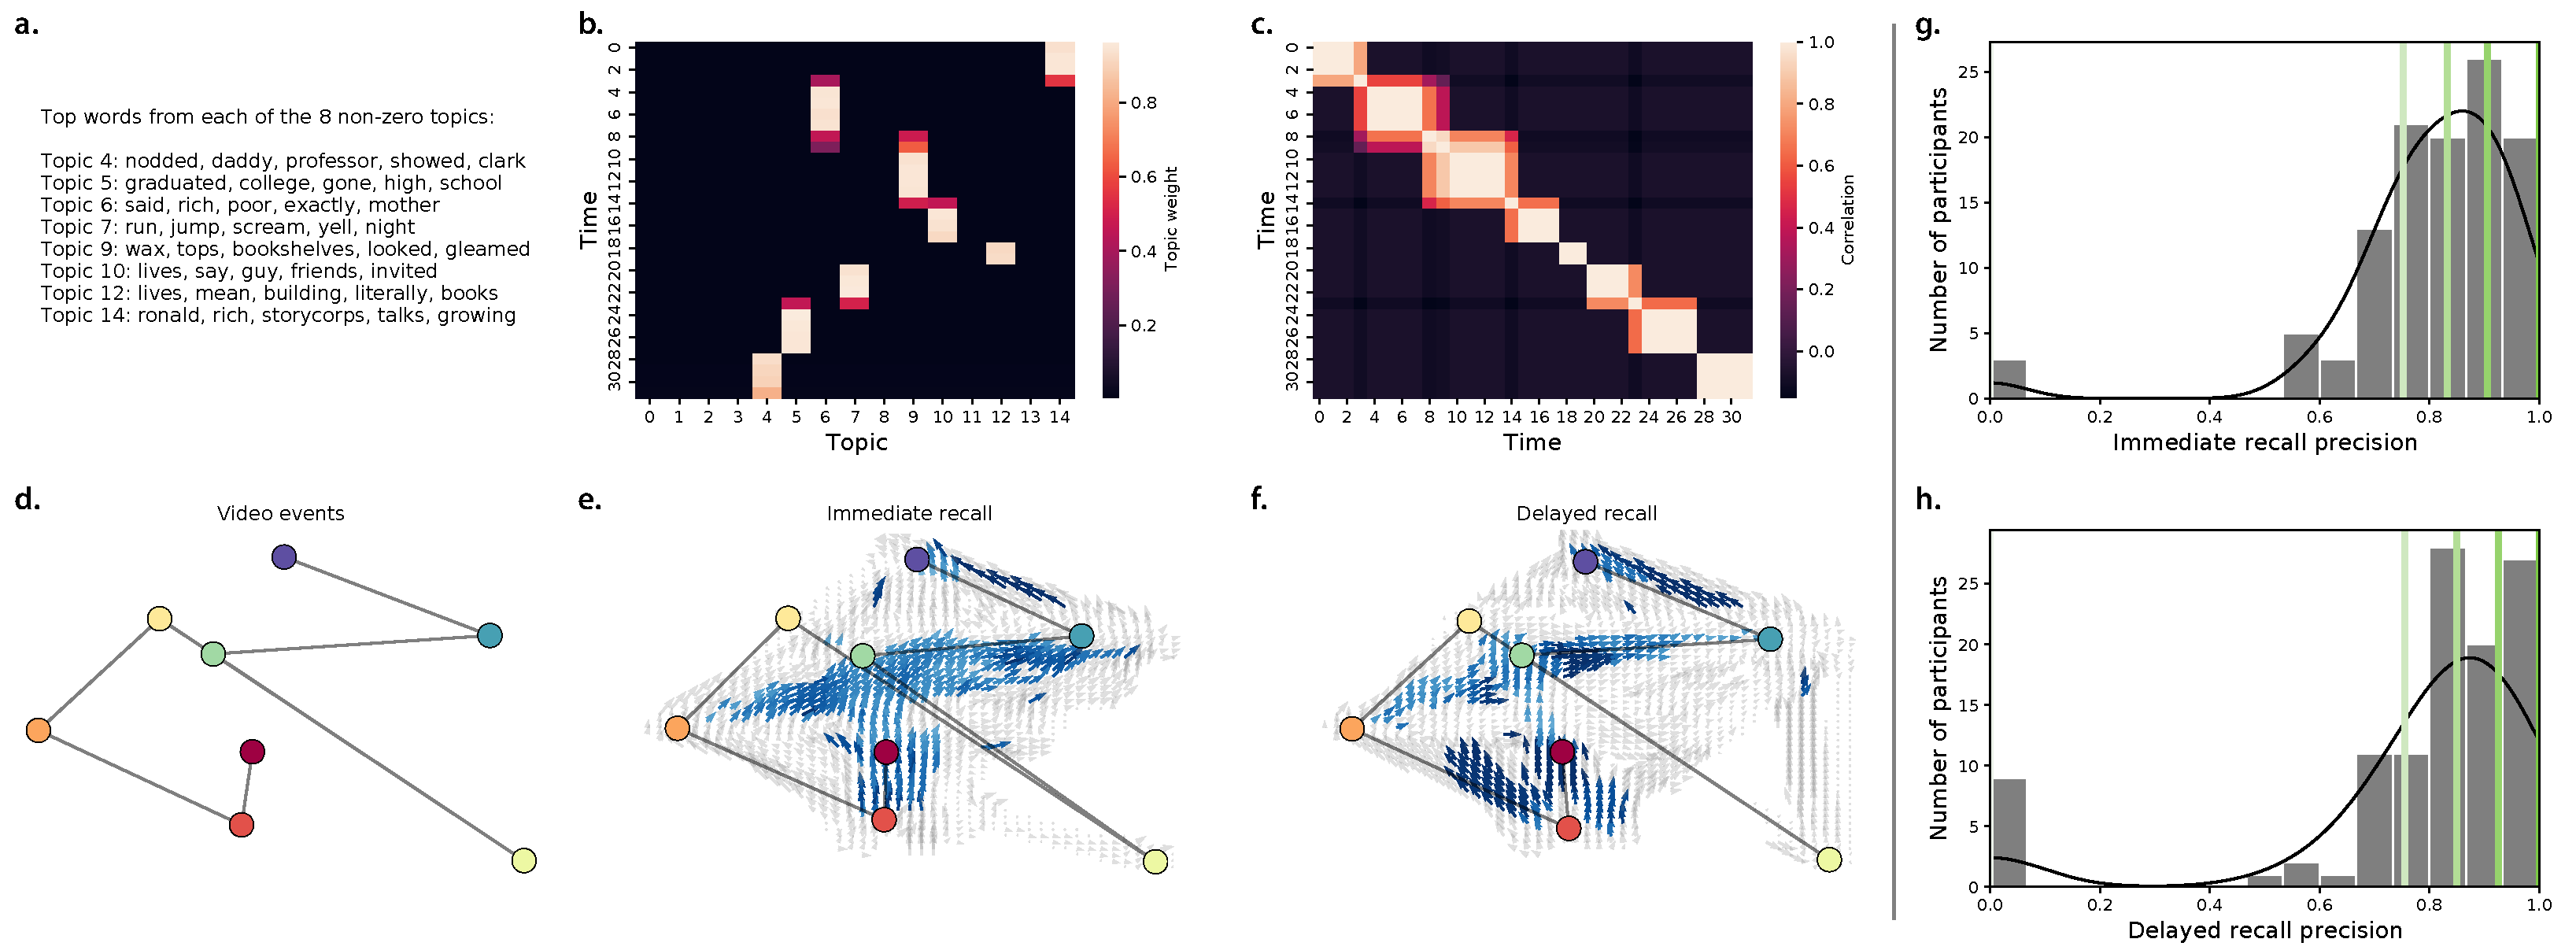
\includegraphics[width=1\textwidth]{figs/naturalistic_recall_behavior}
\caption{\textbf{Naturalistic recall behavioral results.}}
\label{fig:nat_behavioral}
\end{figure}

\begin{figure}[p]
\centering
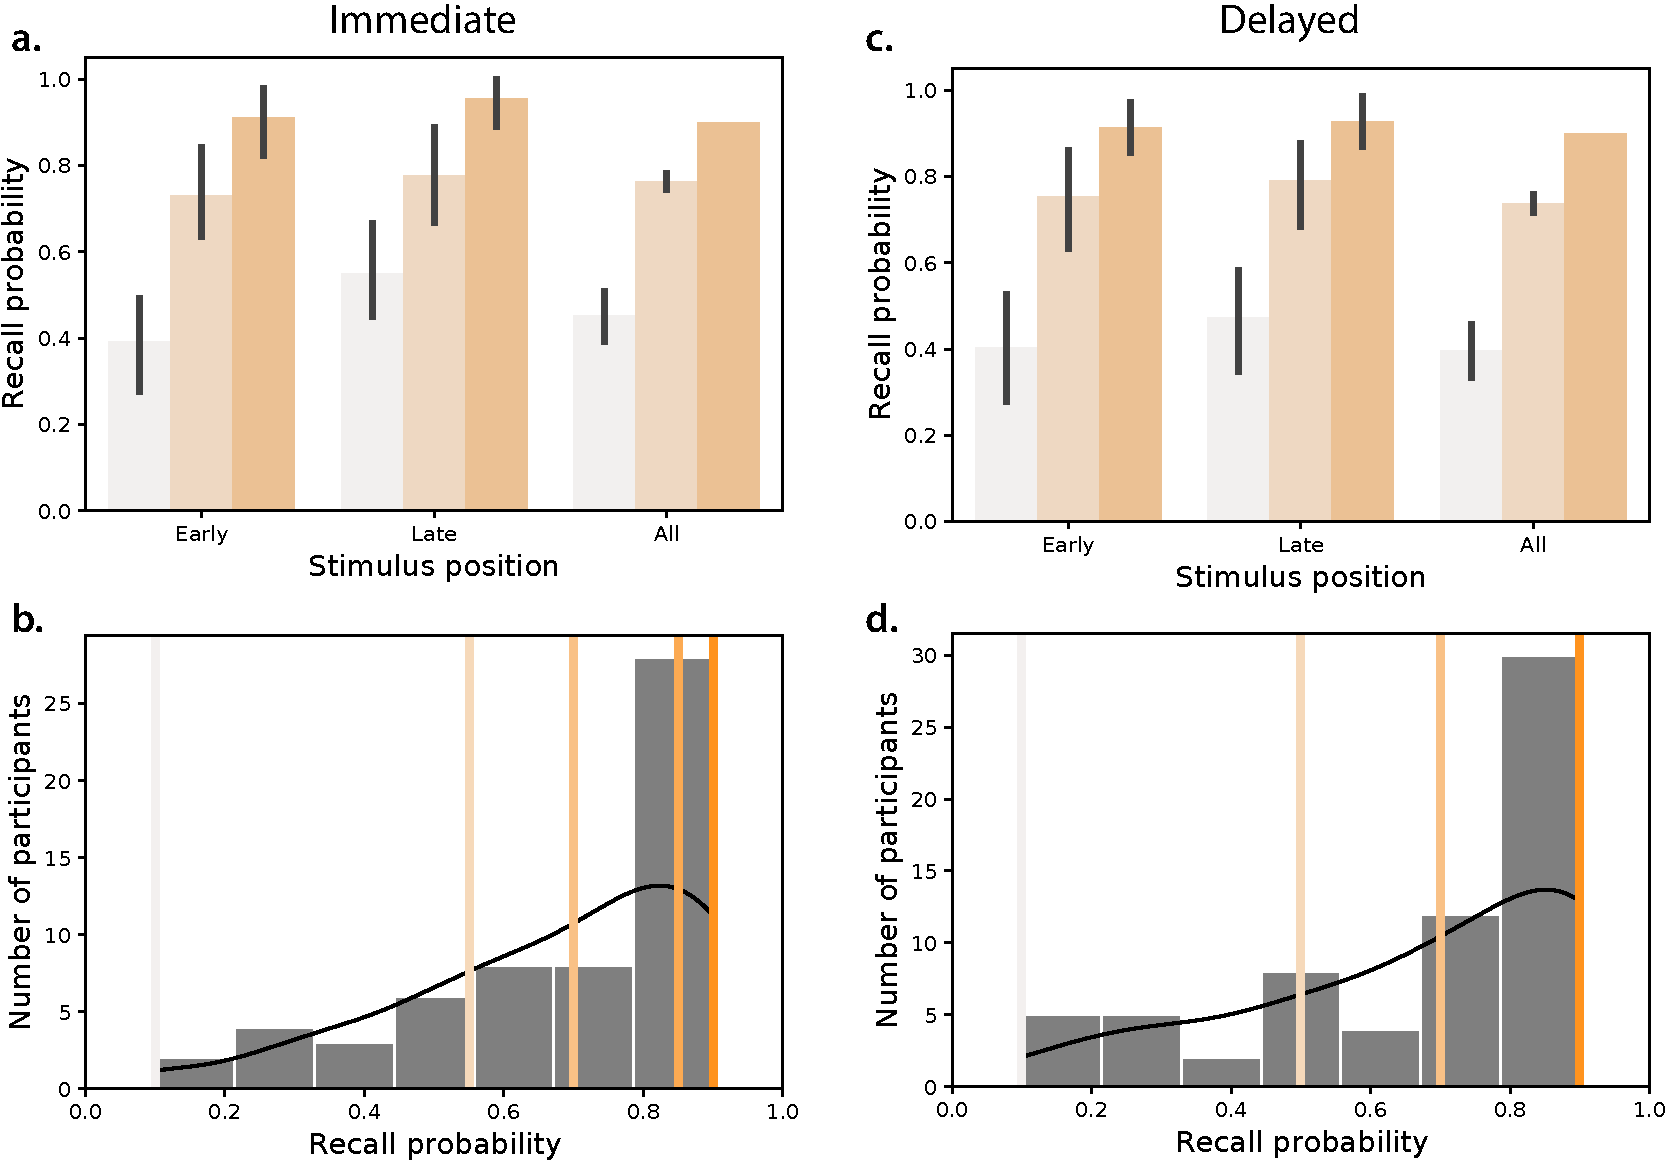
\includegraphics[width=0.6\textwidth]{figs/vocab_learning_behavior}
\caption{\textbf{Foreign language vocabulary learning behavioral results.}}
\label{fig:vocab_behavioral}
\end{figure}

\begin{figure}[p]
\centering
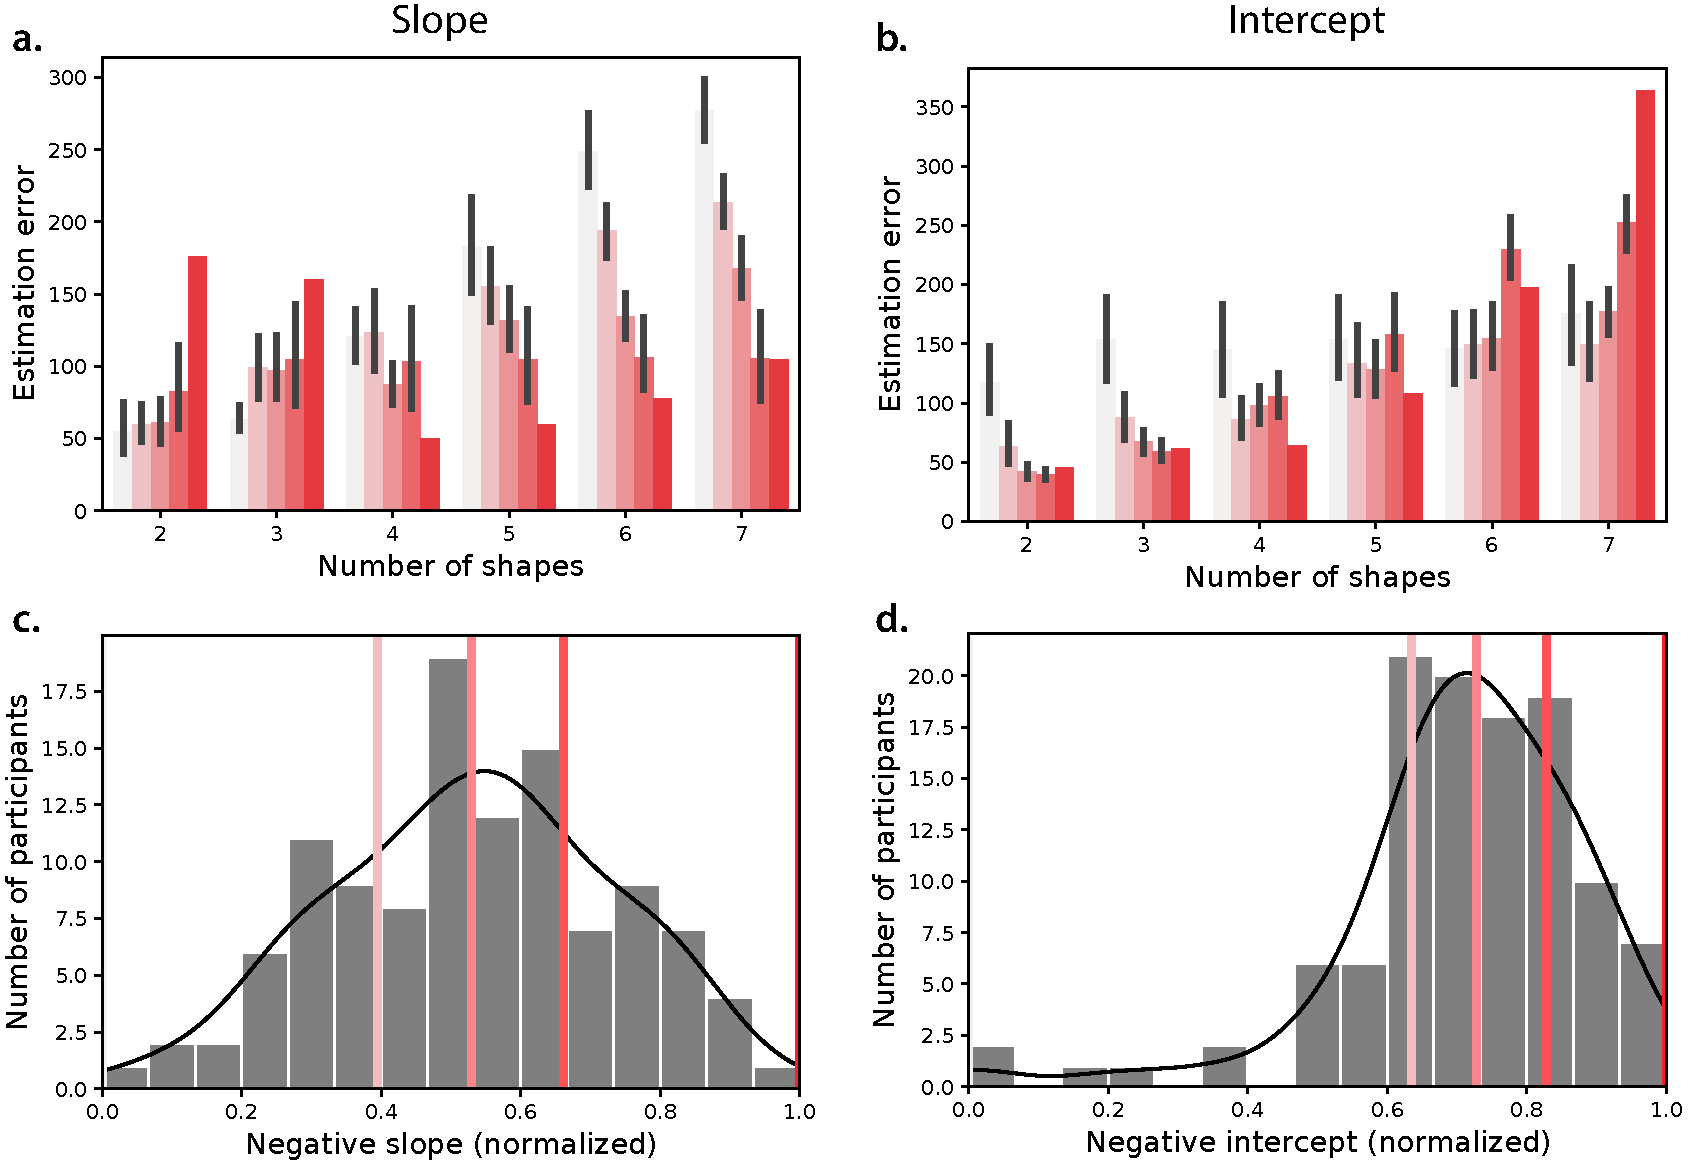
\includegraphics[width=0.6\textwidth]{figs/spatial_learning_behavior}
\caption{\textbf{Spatial learning behavioral results.}}
\label{fig:spatial_behavioral}
\end{figure}



\bibliographystyle{apa}
\bibliography{/Users/jmanning/CDL-bibliography/cdl}
\end{document}
